% DO NOT COMPILE THIS FILE DIRECTLY!
% This is included by the other .tex files.

\section{Timed Automata}
\begin{frame}{Transition System}
\begin{mydef}[Labeled Transition System]
A labeled transition system is a 3-tuple A = $\langle S, Act, s_o \rangle$ where
\begin{itemize}
\item $S$ is a finite set of states
\item $Act$ is a finite set of labelled actions
\item $s_o \in S$ is a finite set of actions
\end{itemize}
\end{mydef}
\end{frame}

\begin{frame}{Transition System}
\begin{figure}
\begin{tikzpicture}[->,>=stealth',shorten >=1pt,auto,node distance=3cm,
                    thick,main node/.style={circle,draw}]

  \node[main node] (1) {1};
  \node[main node] (2) [right of=1] {2};
  \node[main node] (3) [right of=2] {3};
  
\end{tikzpicture}
\end{figure}
\end{frame}

\begin{frame}{Transition System}
\begin{figure}
\begin{tikzpicture}[->,>=stealth',shorten >=1pt,auto,node distance=3cm,
                    thick,main node/.style={circle,draw}]

  \node[main node] (1) {1};
  \node[main node] (2) [right of=1] {2};
  \node[main node] (3) [right of=2] {3};

  \path[every node/.style={font=\sffamily\small}]
    (1) edge node [above] {\EUR{0.50}} (2)
        edge [bend left] node[above] {\EUR{1.00}} (3)
    (2) edge node [above] {\EUR{0.50}} (3)
    (3) edge [bend left] node [below] {coffee} (1);

\end{tikzpicture}
\end{figure}
\end{frame}

\begin{frame}{Transition System}
\begin{figure}
\begin{tikzpicture}[->,>=stealth',shorten >=1pt,auto,node distance=3cm,
                    thick,main node/.style={circle,draw}]

  \node[initial, main node] (1) {1};
  \node[main node] (2) [right of=1] {2};
  \node[main node] (3) [right of=2] {3};

  \path[every node/.style={font=\sffamily\small}]
    (1) edge node [above] {\EUR{0.50}} (2)
        edge [bend left] node[above] {\EUR{1.00}} (3)
    (2) edge node [above] {\EUR{0.50}} (3)
    (3) edge [bend left] node [below] {coffee} (1);
\end{tikzpicture}
\end{figure}
\end{frame}


\begin{frame}{Timed Automata}
\begin{mydef}[Timed Automata]
\label{def:TA}
An extended timed automaton is a 6-tuple A = $\langle L, C, Act, l_0, \rightarrow, I_c\rangle$ where
	\begin{itemize}
		\item L is a finite set of locations, typically denoted by $l$
		\item C is a finite set of clocks, typically denoted by c
		\item Act is a finite set of actions
		\item $l_0 \in$ L is the initial location
		\item $\rightarrow \subseteq L \times G(C) \times Act \times 2^C \times L$ is the (non-deterministic) transition relation.
		\item $I_C : L \rightarrow G(C)$ is a function mapping locations to downwards closed clock invariants.
	\end{itemize}
\end{mydef}
\end{frame}

\begin{frame}{Timed Automata}
\includegraphics[width=\textwidth]{img/TA}
\end{frame}


\section{Symbolic Model Checking}

\begin{frame}{Boolean Decision Diagram}
	\begin{itemize} 
		\item Expresses boolean expressions \pause
		\item States can be seen as boolean expressions \pause
		\item Memory efficient
	\end{itemize} 
\end{frame}

\begin{frame}{Boolean Decision Diagram}
\begin{figure}[h]
\centering
	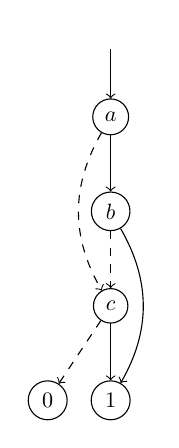
\begin{tikzpicture}[
		smallvertex/.style={circle,draw,scale=0.8}
		]
		\node[smallvertex](S1){$a$};
		\node[smallvertex, draw = none, above of = S1, yshift = 0.25cm](S0){};
		
		\node[smallvertex, below of = S1, yshift = -.5cm](S2){$b$};
		\node[smallvertex, below of = S2, yshift = -.5cm](S3){$c$};
		\node[smallvertex, below of = S3, yshift = -.5cm](S4){$1$};
		\node[smallvertex, left of = S4](S5){$0$};
		
		\draw[->] (S0) --(S1) node [midway, above, sloped, scale=0.75,
		rotate=0, xshift =-0.4 cm, yshift = -0.2cm]{};
		\draw[->] (S1) --(S2) node [midway, above, sloped, scale=0.75,
		rotate=90, xshift =-0.4 cm, yshift = -0.2cm]{};
		\draw[dashed,->] (S2) --(S3) node [midway, above, sloped, scale=0.75,
		rotate=90, xshift =-0.4 cm, yshift = -0.2cm]{};
		\draw[->] (S3) --(S4) node [midway, above, sloped, scale=0.75,
		rotate=90, xshift =-0.4 cm, yshift = -0.2cm]{};		
		\draw[->,dashed] (S1) edge[bend right](S3) node [midway, above, sloped, scale=0.75,
		rotate=90, xshift =-0.4 cm, yshift = -0.2cm]{};	
		\draw[->] (S2) edge[bend left](S4) node [midway, above, sloped, scale=0.75,
		rotate=90, xshift =-0.4 cm, yshift = -0.2cm]{};	
		\draw[dashed,->] (S3) --(S5) node [midway, above, sloped, scale=0.75,
		rotate=90, xshift =-0.4 cm, yshift = -0.2cm]{};
		[bend left]
	\end{tikzpicture}
\caption{A BDD representing $(a \wedge b) \vee c$}
\label{fig:BDD}
\end{figure}
\end{frame}

\begin{frame}{List Decision Diagram}
\begin{figure}
	\begin{tikzpicture}[
		smallvertex/.style={circle,draw,scale=0.8}
		]
		\node[smallvertex, draw = none, above of = S1, yshift = 0.25cm](S0){};
		\node[smallvertex](S1){$a$};
		\node[smallvertex, below of = S1, yshift = -.5cm](S2){$b$};
		\node[smallvertex, below of = S2, yshift = -.5cm](S3){$c$};
		\node[smallvertex, below of = S3, yshift = -.5cm](S4){$d$};
		\node[smallvertex, below of = S4, yshift = -.5cm](S5){$T$};
		\node[smallvertex, right of = S2](S6){$b$};
		\node[smallvertex, right of = S3](S7){$c$};
		\node[smallvertex, right of = S6](S9){$b$};
		\node[smallvertex, above of = S9, yshift = .5cm](S8){$a$};
		\node[smallvertex, below of = S9, yshift = -.5cm](S10){$c$};
		\node[smallvertex, below of = S10, yshift = -.5cm](S11){$d$};
		
		\draw[->] (S0) --(S1) node [midway, above, sloped, scale=0.75,
		rotate=0, xshift =-0.4 cm, yshift = -0.2cm]{};
		\draw[->] (S1) --(S2) node [midway, above, sloped, scale=0.75,
		rotate=90, xshift =-0.4 cm, yshift = -0.2cm]{$0$};
		\draw[->] (S2) --(S3) node [midway, above, sloped, scale=0.75,
		rotate=90, xshift =-0.4 cm, yshift = -0.2cm]{$0$};
		\draw[->] (S3) --(S4) node [midway, above, sloped, scale=0.75,
		rotate=90, xshift =-0.4 cm, yshift = -0.2cm]{$0$};
		\draw[->] (S4) --(S5) node [midway, above, sloped, scale=0.75,
		rotate=90, xshift =-0.4 cm, yshift = -0.2cm]{$0$};
		\draw[dashed, ->] (S2) --(S6) node [midway, above, sloped, scale=0.75,
		rotate=90, xshift =-0.4 cm, yshift = -0.2cm]{};
		\draw[->] (S6) --(S7) node [midway, above, sloped, scale=0.75,
		rotate=90, xshift =-0.4 cm, yshift = -0.2cm]{$2$};
		\draw[->] (S7) --(S4) node [midway, above, sloped, scale=0.75,
		rotate=300, xshift =0.4 cm, yshift = -0.2cm]{$3$};
		\draw[dashed, ->] (S1) --(S8) node [midway, above, sloped, scale=0.75,
		rotate=90, xshift =-0.4 cm, yshift = -0.2cm]{};
		\draw[->] (S8) --(S9) node [midway, above, sloped, scale=0.75,
		rotate=90, xshift =-0.4 cm, yshift = -0.2cm]{$2$};
		\draw[->] (S9) --(S10) node [midway, above, sloped, scale=0.75,
		rotate=90, xshift =-0.4 cm, yshift = -0.2cm]{$0$};
        \draw[->] (S10) --(S11) node [midway, above, sloped, scale=0.75,
		rotate=90, xshift =-0.4 cm, yshift = -0.2cm]{$3$};
		\draw[->] (S11) --(S5) node [midway, above, sloped, scale=0.75,
		rotate=320, xshift =-0.4 cm, yshift = -0.2cm]{$1$};


	\end{tikzpicture}
\label{fig:ldd-example}
\end{figure}
\end{frame}

\section{LTSmin}

\section{Working with \LaTeX}
\begin{frame}{Font Sizes}
  \begin{table}[htdp]
\caption{The different font sizes within \LaTeX}
\begin{center}
\begin{tabular}{| l c |} \hline
 tiny			& {\tiny sample text}\\
 scriptsize		& {\scriptsize sample text}\\
 footnotesize	& {\footnotesize sample text}\\
 small		& {\small sample text}\\
 normalsize	& {\normalsize sample text}\\
 large		& {\large sample text}\\
 Large 		& {\Large sample text}\\
 LARGE 		& {\LARGE sample text}\\
 huge 		& {\huge sample text}\\
 Huge		& {\Huge sample text} \\\hline

\end{tabular}
\end{center}
\label{default}
\end{table}%
\end{frame}

\begin{frame}{Creation of a new frame}
The text within the frame
\end{frame}


\frame[containsverbatim]{\frametitle{Creation of a new frame - \texttt{source}}% 
\begin{verbatim} 

\begin{frame}{Creation of a new frame}
    The text within the frame
\end{frame}

\end{verbatim} 
}% 
	
\begin{frame}{Frame with \texttt{pause} itemes}
	\begin{itemize} 
		\item First item \pause
		\item Second item \pause
		\item You get the point. 
	\end{itemize} 
\end{frame}


\frame[containsverbatim]{\frametitle{Frame with \texttt{pause} itemes - \texttt{source}}% 
\begin{verbatim} 

\begin{frame}{Frame with \texttt{pause} itemes}
	\begin{itemize} 
		\item First item \pause
		\item Second item \pause
		\item You get the point. 
	\end{itemize} 
\end{frame}

\end{verbatim} 
}% 


\begin{frame}{Frame with \texttt{pause} tables}
	
	\rowcolors[]{1}{blue!20}{blue!10} 
	\begin{table}
	\caption{Caption}
	\begin{tabular}{l!{\vrule}cccc}  
		Class & A & B & C & D \\\hline 
		X & 1 & 2 & 3 & 4 \pause \\ 
		Y & 3 & 4 & 5 & 6 \pause \\ 
		Z & 5 & 6 & 7 & 8 
	\end{tabular}
	\end{table}
\end{frame}



\frame[containsverbatim]{\frametitle{Frame with \texttt{pause} tables - \texttt{source}}% 
\begin{verbatim} 
\begin{frame}{Frame with \texttt{pause} tables}
	
	\rowcolors[]{1}{blue!20}{blue!10} 
	\begin{table}
	\caption{Caption}
	\begin{tabular}{l!{\vrule}cccc}  
		Class & A & B & C & D \\\hline 
		X & 1 & 2 & 3 & 4 \pause \\ 
		Y & 3 & 4 & 5 & 6 \pause \\ 
		Z & 5 & 6 & 7 & 8 
	\end{tabular}
	\end{table}
\end{frame}


\end{verbatim} 
}% 



\begin{frame}{Two Column Output} 
  \begin{columns}[c] 
    \column{1.5in} 
      Text here.\\ 
      Text here.\\ 
      Text here.
    \column{1.5in} 
    \framebox{\includegraphics[width=1.5in]{img/back2EN}} 
  \end{columns} 
\end{frame} 



\frame[containsverbatim]{\frametitle{Two Column Output - \texttt{source}}% 
\begin{verbatim} 
\begin{frame}{Two Column Output} 
  \begin{columns}[c] 
    \column{1.5in} 
      Text here.\\ 
      Text here.\\ 
      Text here.
    \column{1.5in} 
    \framebox{\includegraphics[width=1.5in]{img/back2}} 
  \end{columns} 
\end{frame} 


\end{verbatim} 
}% 


\section{Second Section}

\begin{frame}{First frame of the Second Section} 
Each new section starts with an Table Of Contents.
\end{frame} 

\section{Third Section}
\begin{frame}{First frame of the Second Section} 
The Table Of Contents is clickable
\end{frame} 
